% \documentclass{article}
% \usepackage{tikz}
% \usetikzlibrary{arrows.meta, positioning}

\documentclass[a4paper,12pt]{article}
\usepackage[margin=1in]{geometry}
\usepackage{tikz}
\usetikzlibrary{arrows.meta, positioning}

\begin{document}

\begin{center}
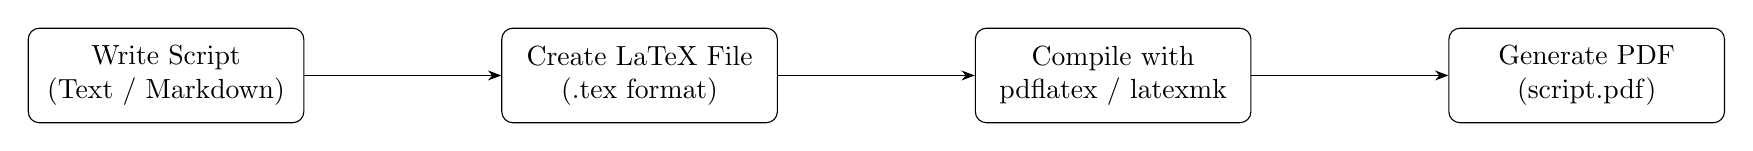
\begin{tikzpicture}[
    node distance=1.5cm and 2.5cm,
    box/.style={draw, rectangle, rounded corners, align=center, minimum width=3.5cm, minimum height=1.2cm},
    ->, >=Stealth
]

\node[box] (script) {Write Script\\(Text / Markdown)};
\node[box, right=of script] (latex) {Create LaTeX File\\(.tex format)};
\node[box, right=of latex] (compile) {Compile with\\pdflatex / latexmk};
\node[box, right=of compile] (pdf) {Generate PDF\\(script.pdf)};

\draw[->] (script) -- (latex);
\draw[->] (latex) -- (compile);
\draw[->] (compile) -- (pdf);

\end{tikzpicture}
\end{center}

\end{document}


